\chapter{Wykład 7. Zintegrowane zarządzanie projektem informatycznym}

\section{Sukces projektu}
% strona 23

\subsection*{Definicja sukcesu projektu}
	Realizowany projekt poprzez pozyskanie sponsora, ma z góry ustalony budżet, którego nie może przekroczyć. Niewielki wzrost kosztów jest akceptowalny, jednak spowoduje on zmniejszenie zysków dla firmy. Nieakceptowalna jest sytuacja, w której koszty przekroczą zyski a nasze przedsiębiorstwo będzie stratne. Możliwe jest przekroczenie terminu realizacji nawet o 50\%. Powyżej tej granicy, może się okazać, że sytuacja na rynku ulegnie zmianie a stworzona aplikacja przestanie być atrakcyjna dla klientów i nie uzyska poziomu spodziewanej sprzedaży i przyniesie straty. Zakres projektu ustalony z klientem nie może zostać uszczuplony. Podsumowując, projekt zakończy się sukcesem w przypadku, gdy uda się zachować zakres projektu oraz koszty na zakładanym poziomie, pomimo przekroczenia planowanego czasu realizacji nawet o połowę.

\begin{table}[htb]
\centering
\begin{tabular}{l|p{7cm}}
		Rodzaj sukcesu & Opis sukcesu \\
\hline
\hline
		Główny & koszt dostarczenia produktu nie przekroczy zakładanego poziomu \\
\hline
		Uzupełniający & produkt będzie realizował wszystkie zgłoszone przez klienta wymagania \\
\hline
		Uzupełniający & produkt po wypuszczeniu na rynek osiągnie przewidywany poziom sprzedaży \\
\hline
\end{tabular}	
	\caption{Definicja sukcesu}
	\label{tab:defSukcesu}
\end{table}

\subsection*{Model NTCP produktu}
	Model NTCP ilustruje na czym opiera się sukces naszego projektu. Tworzony jest nowatorski (nie ma drugiego takiego na rynku) system, częściowo wykorzystujący istniejące technologie. Czas realizacji projektu nie jest najistotniejszy, jednak ważne jest, by zdążyć przed konkurencją, inaczej rynek zbytu ulegnie skurczeniu.
\begin{figure}[!h]
\centering
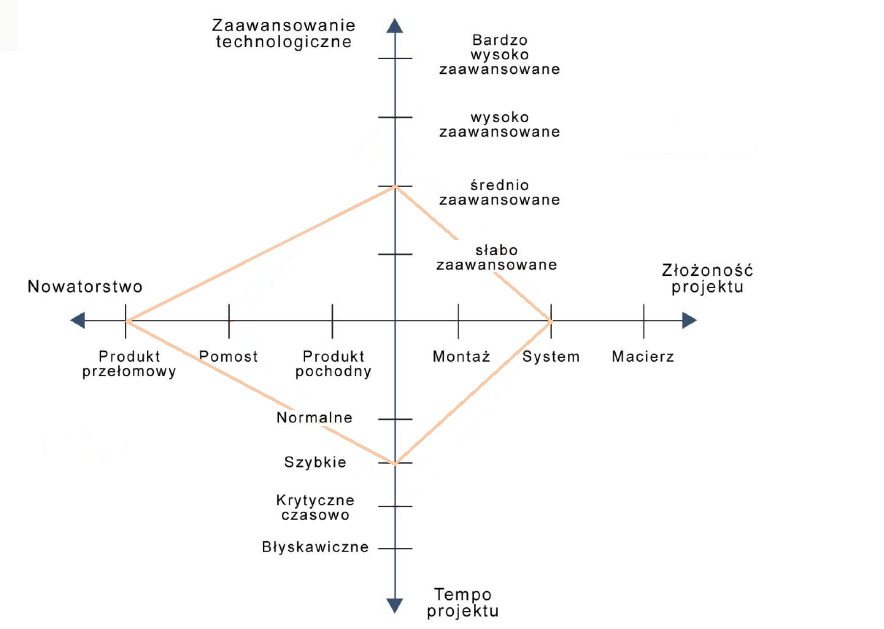
\includegraphics[width=\textwidth]{ntpc}
\caption{Model NTCP}
\label{ntpc}
\end{figure}

% ===========================================================================

\section{Rozpoczęcie projektu}
% strona 28
Decyzja o podjęciu prac nad projektem została przedstawiona w postaci deklaracji prac projektu.
\subsection*{Deklaracja prac projektu}
\begin{enumerate}
	\item \textbf{Powód:} Ideą przedsięwzięcia jest stworzenie systemu pomagającego przedsiębiorstwom zarządzać projektami zgodnie z metodyką PMBOK. Naszym celem jest utworzenie dochodowego systemu, jaki do tej pory nie pojawił się na rynku. Wiele przedsiębiorstw nie korzysta z żadnej metodyki w pracy swojej firmy, przez co traci wiele zasobów na uzupełnienie tych braków i uzyskuje gorsze osiągi na tle swojej konkurencji. Dzięki proponowanemu systemowi stosowanie metodyki PMBOK w firmie stanie się dużo prostsze, a zyski stosujących go przedsiębiorstw wymiernie wzrosną. PMBOK jest popularną metodyką o szerokim zastosowaniu, stąd prawdopodobieństwo odniesienia sukcesu jest wysokie.
	\item \textbf{Opis prac:} Nasza firma będzie odpowiedzialna za analizę systemu, projekt, implementację, testy oraz wdrożenie i szkolenia nowych użytkowników systemu. Wszystkie etapy będą się opierały o wymagania dostarczone przez klienta. Efektem końcowym projektu będzie zaawansowany system wspierający realizację projektów z wykorzystaniem metodyki PMBOK.
	\item \textbf{Miejsce wykonywania:} Siedziba naszej firmy.
	\item \textbf{Okres prac:} 12-03-2012 do 01-12-2012
	\item \textbf{Kamienie milowe:}
		\begin{itemize}
			\item Spotkanie wprowadzające, do 12-03-2012
			\item Analiza wymagań, do 22-03-2012
			\item Projekt techniczny, do 02-05-2012
			\item Rozpoczęcie implementacji systemu, do 12-06-2012
			\item Testowanie, do 01-10-2012
			\item Wypuszczenie produktu na rynek, do 01-12-2012
		\end{itemize}
	\item \textbf{Wymagania:}  Aby nasz produkt stał się użyteczny należy zebrać opinie ekspertów - osób zajmujących się zarządzaniem projektami i dowiedzieć się, w jakich aspektach zarządzania potrzebne jest największe wsparcie i na co należy zwrócić szczególną uwagę. Potrzebujemy również pozyskać reklamodawców, aby zainteresować potencjalnych klientów naszym produktem.
	\item \textbf{Kryteria akceptacji:}  Wysoka popularność systemu, pozyskanie reklamodawców i nie przekroczenie budżetu.
\end{enumerate}

% ===========================================================================

\section{Karta projektu}
Kartę projektu została przedstawiona na kolejnych stronach.
% strona 33
\begin{figure}[!h]
\centering
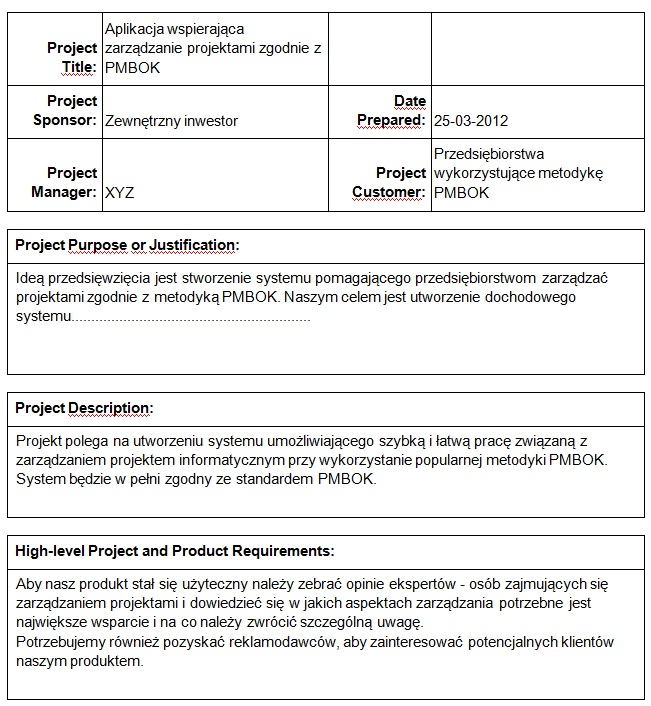
\includegraphics[width=\textwidth]{kartaProjektu1}
\caption{Karta projektu cz.1}
\label{kartaProjektu1}
\end{figure}

\begin{figure}[!h]
\centering
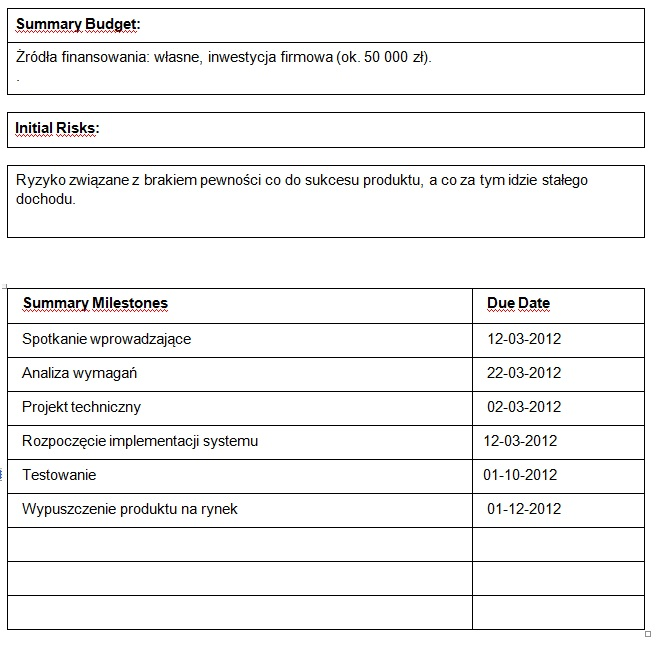
\includegraphics[width=\textwidth]{kartaProjektu2}
\caption{Karta projektu cz.2}
\label{kartaProjektu2}
\end{figure}

\begin{figure}[!h]
\centering
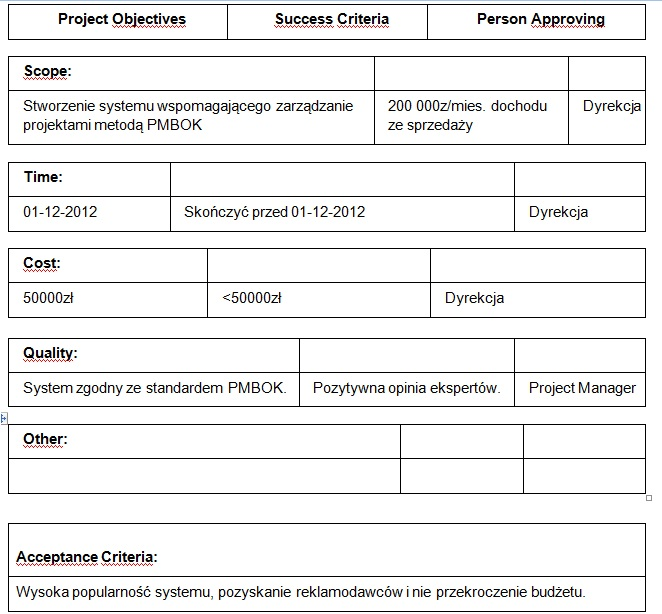
\includegraphics[width=\textwidth]{kartaProjektu3}
\caption{Karta projektu cz.3}
\label{kartaProjektu3}
\end{figure}

\begin{figure}[!h]
\centering
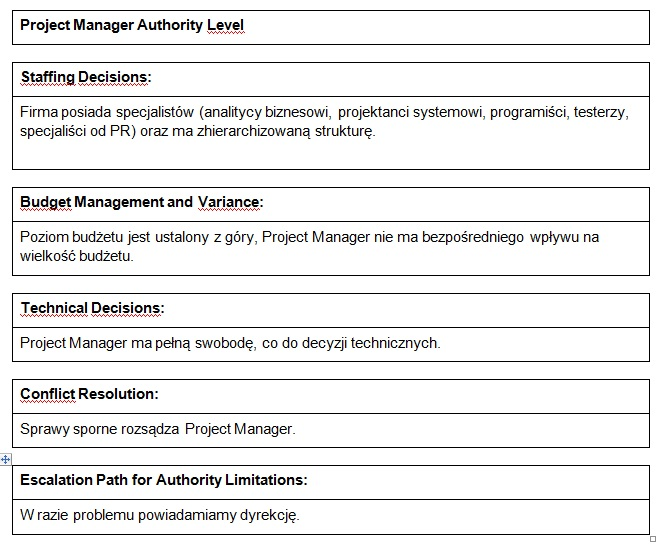
\includegraphics[width=\textwidth]{kartaProjektu4}
\caption{Karta projektu cz.4}
\label{kartaProjektu4}
\end{figure}

\clearpage

% ===========================================================================

\section{Plan zarządzania projektem wg B.A.R.F.}
% strona 44

Plan uzgodniony z wszystkimi, zaakceptowany, możliwy do realizacji oraz formalny. W procesie uzgadniania planu zarządzania projektem byli obecni wszyscy interesariusze projektu. Nikt nie zgłosił sprzeciwu wobec uzgadnianych treści, dlatego plan spełnia kryteria uzgodnienia z wszystkimi i akceptowalności. Plan uwzględnia jedynie procedury, które będą stosowane podczas wykonywania projektu dzięki czemu jest możliwy do realizacji a wszystkie dokumenty (wnioski, uwagi, raporty) mają ściśle określony schemat spełniając kryterium formalności.

\subsection*{Cel dokumentu}
Celem dokumentu jest opisanie wszystkich czynności związanych z zarządzaniem projektem. Służy on także do wspomagania organizacji całego procesu projektowego i przygotowania grupy projektowej do efektywnej pracy. Dokument powstanie przy współpracy wszystkich najważniejszych interesariuszy mających duży wpływ lub zainteresowanie projektem.

\subsection*{Zakres}
Dokument ten obejmuje wszystkie elementy mające istotny wpływ na zarządzanie projektem.
Na jego całokształt składa się szereg dokumentów:
\begin{itemize}
	\item Opis projektu
	\item Plan zarządzania wymaganiami
	\item Plan kontroli harmonogramu
	\item Plan komunikacji
	\item Plan zarządzania konfiguracją
	\item Plan zarządzania zmianą
	\item System kontroli zmian
	\item System autoryzacji pracy
\end{itemize}
Treść dokumentu może zostać zaktualizowany na kolejnych etapach realizacji projektu.

\subsection*{Opis projektu}
Celem projektu jest stworzenie złożonego systemu informatycznego umożliwiającego zarządzanie projektami z wykorzystaniem metodyki PMBOK. Projekt ma z góry ustalony budżet oraz koszty, które nie powinny zostać przekraczane, aby przedsięwzięcie zakończyło się sukcesem.

\subsection*{Plan zarządzania wymaganiami}
\begin{itemize}
	\item Identyfikacja - Wymagania będą identyfikowane podczas wspólnych spotkań zespołu projektowego, klienta oraz specjalistów w dziedzinie metodyki PMBOK. Celem takich spotkań będzie formalizacja uzgodnień dotyczących funkcjonalności tworzonej aplikacji.
	\item Zarządzanie wymaganiami - Zidentyfikowane wymagania muszą zostać zaakceptowane przez wszystkich interesariuszy projektu. Zadaniem Project Menagera jest dopilnowanie, aby klient, inwestor oraz zespół projektowy wyrazili aprobatę zdefiniowanych wymagań. Wszelkie zmiany wprowadzane w wymaganiach również muszą zostać zaakceptowane przez najważniejszych interesariuszy aby mogły zostać zrealizowane w systemie.
	\item Kontrola wymagań - W celu zapewnienia kontroli nad wymaganiami, do każdego zidentyfikowanego wymagania zostaną wymienione dodatkowe reguły lub wskazówki niezbędne do zastosowania w celu śledzenia powiązań z innymi wymaganiami. Główną zasadą, która zagwarantuje kontrolę jest to, że każda zaakceptowana cecha oprogramowania musi być powiązana przynajmniej z jednym przypadkiem użycia lub przynajmniej z jednym wymaganiem dodatkowym. W ten sposób łatwo będzie można skontrolować czy wszystkie zidentyfikowane wymagania zostały uwzględnione w systemie.
\end{itemize}

\subsection*{Plan kontroli harmonogramu}
Po zakończeniu każdej fazy kierownik będzie sprawdzał na podstawie raportów weryfikujących postęp i zgodność projektu z planem. Kierownik w razie konieczności będzie wprowadzał na bieżąco korekty do planu, modyfikując odpowiednie dokumenty, i powiadamiając klientów oraz członków zespołu o zaistniałych korektach. Każda zmiana w harmonogramie zostanie zatwierdzona przez kierownika funkcyjnego dysponującego zasobami oraz zespół projektowy.


\subsection*{Plan komunikacji}
	Zgłaszanie zmian w projekcie odbywać się będzie poprzez wypełnienie wniosku zmiany i przesłanie go do Project Managera. Każde zgłoszenie opatrzone będzie informacją o dacie złożenia zgłoszenia, zgłaszającym oraz wprowadzającym zgłoszenie do systemu, priorytecie zgłoszenia (poważny błąd aplikacji czy drobna zmiana funkcjonalna), tytułem, opisem zgłoszenia, informacją o wersji produktu, którego dotyczy zmiana oraz stopniu jego realizacji (przyjęte, zgłoszone do akceptacji, przyjęte/odrzucone, zrealizowane). Każda modyfikacja stanu zgłoszenia będzie kończona poprzez przesłanie informacji do składającego wniosek. 

	Aktualne postępy prac będą zapisywane przy pomocy Raportów Stanów Prac. Określone w nich będą informacje dotyczące zakresu prace jakie miały zostać wykonane na danym etapie, osobę odpowiedzialną oraz co udało się zrealizować. Dodatkowo może zawierać informacje dotyczące problemów powstałych przy próbie wykonania danego zadania.

\subsection*{Plan zarządzania konfiguracją}
\begin{itemize}
	\item Identyfikacja konfiguracji - Najważniejszym elementem konfiguracji są kolejne wersje oprogramowania. Mniej ważne, ale również konieczne jest zarządzanie konfiguracją dokumentacji technicznej. Każda pozycja konfiguracji musi być jednoznacznie określona, co zostanie zapewnione poprzez nadawanie niepowtarzalnych identyfikatorów. Zastosowana konwencja identyfikacji będzie odzwierciedlać hierarchiczną oraz chronologiczną strukturę konfiguracji, rodzaj pozycji i/lub przypisanie pozycji do projektu. 
	\item Zarządzanie konfiguracją - Wszystkie elementy wchodzące w skład konfiguracji systemu zostaną umieszczone w systemie kontroli wersji GIT. Kolejne wersje oprogramowania oraz dokumentacji będą przechowywane we wspólnym repozytorium, do którego dostęp będą mieli jedynie członkowie zespołu projektowego. Wszelkie zmiany będą opisywane krótkim komentarzem, co zostało zmienione, oraz podpisane imieniem i nazwiskiem osoby wprowadzającej zmiany. 
	\item Weryfikacja - Kontrolę nad zarządzaniem konfiguracją sprawować będą inżynierowie jakości. Ich zadaniem będzie weryfikowanie czy w aktualnej wersji oprogramowania zostały uwzględnione najnowsze poprawki i zmiany.
\end{itemize}

\subsection*{Plan kontroli zmian}
Plan kontroli zmian określa szereg czynności, które zostaną wykonane po zgłoszeniu żądania zmiany w projekcie. Kontrola zmian składać się będzie z następujących etapów:
\begin{enumerate}
	\item Złożenie wniosku o zmianę poprzez wypełnienie formularza i wysłanie go do managera zmian (w tym przypadku Project Managera).
	\item Project Manager wprowadza otrzymany wniosek do spisu żądań zmian. Status wniosku jest aktualizowany na każdym etapie jego rozpatrywania.
	\item Zespół projektowy rozpatruje wniosek pod kątem nakładów jakich wymagało będzie wprowadzenie żądanej zmiany oraz proponuje rozwiązanie realizujące daną zmianę.
	\item Podjęcie decyzji o opłacalności wprowadzenia żądanej zmiany.
	\item Jeśli decyzja jest pomyślna, następuje etap dokładnego zaplanowania wprowadzanej zmiany oraz jej implementacja. Następuje również powiadomienie składającego wniosek o jego pozytywnym rozpatrzeniu oraz poinformowanie wszystkich interesariuszy, że system ulegnie zmianie.
\end{enumerate}

\subsection*{System kontroli zmian}
Zewnętrzny system, w którym zapisywane będą wszystkie zgłaszane żądania zmian. Każde zgłoszenie opatrzone będzie informacją o dacie złożenia zgłoszenia, zgłaszającym oraz wprowadzającym zgłoszenie do systemu, priorytecie zgłoszenia (poważny błąd aplikacji czy drobna zmiana funkcjonalna), tytułem, opisem zgłoszenia, informacją o wersji produktu, którego dotyczy zmiana oraz stopniu jego realizacji (przyjęte, zgłoszone do akceptacji, przyjęte/odrzucone, zrealizowane). Decyzje o akceptacji wniosków będą podejmowane na spotkaniach najważniejszych interesariuszy.

\subsection*{System autoryzacji pracy}
Każda zaakceptowana zmiana w systemie zostaje następnie rozpisana jako szereg prac do wykonania przez zespół projektowy wraz z podziałem na konkretne osoby odpowiedzialne. Zespół projektowy zostaje poinformowany, że może rozpoczynać prace nad wprowadzoną zmianą. Po wykonaniu przypisanego zadania zostaje ono oznaczone w systemie jako zrealizowane. Zadaniem Project Managera jest dopilnowanie, aby zadania były realizowane zgodnie z przyjętym harmonogramem. Kolejność realizacji zadań jest taka sama jak w przypadku tworzenia nowego systemu: analiza, projektowanie, implementacja, testy a na końcu wdrożenie. Obowiązek dopilnowania prawidłowej kolejności dokonywania zmian również spoczywa na Project Managerze. 


% ===========================================================================

\section{Propozycja sposobu monitorowania kontroli wykonania projektu}
% strona 89
Proces monitorowania kontroli wykonania projektu postanowiliśmy zrealizować przy pomocy zewnętrznego oprogramowania Github umożliwiającego definiowanie zadań i przypisywanie ich do konkretnych osób oraz określaniu czasu ich realizacji. Aplikacja pozwala również na ustalanie kamieni milowych, które pozwolą zorientować się czy realizacja projektu przebiega zgodnie z planem. 
	Zadania definiowane w programie są pobierane z ustalonego wcześniej harmonogramu prac. Dzięki przejrzystemu określeniu zadań, osób odpowiedzialnych oraz terminów ich realizacji w łatwy sposób Project Manager może przewidywać oraz zapobiegać ewentualnym opóźnieniom. Możliwe jest również bieżące monitorowanie zużycia zasobów i natychmiastową reakcję w przypadku gdy są niewykorzystywane lub nadmiernie przeciążone.




